%%% Dealing with type erasures

%%%============================================================================
Templates are powerful tools as they allow the compiler to perform all kinds of
optimizations. In addition they help to avoid virtual function tables and thus
increasing overall performance of a program. 
Template instantiation virtually always goes along with code generation and thus
with an increase in code size. This can cause problems in particular on small
hardware (like ARM based systems) where resources are limited.
Think about the {\tt show\_info} function template in the previous chapter. The
function will be instantiated for every array type passed to it although it does
virtually the same thing for each of them (we see an example of this in the
section below describing the array type erasure). 

A reasonable solution for this problem is the use of type erasures. 
\libpnicore\ provides three different type erasures
\begin{center}
\begin{tabular}{l | l}
{\tt value} & stores a single scalar value of a POD type \\
{\tt value\_ref} & stores the reference to an instance of a POD type \\
{\tt arra} & stores a multidimensional array type 
\end{tabular}
\end{center}
To use type erasures include the {\tt /pni/core/type\_erasures.hpp} at the top of
your source file.

%%%============================================================================
\section{The {\tt value} type erasures}

The {\tt value} type erasure stores the value of a single scalar POD type. 
{\tt value} can be default constructed in which case an instance of type 
{\tt none} is stored as can be easily confirmed with
\begin{cppcode}
value v;
std::cout<<v.type_id()<<std::endl; //output NONE
\end{cppcode}
{\tt value} has a copy and move constructor for other instances from 
{\tt value}. However, the constructor for other variables and literals is 
explicit 
\begin{cppcode}
//explicit construction from a variable
int32 n = 1000;
value v1(n);     
std::cout<<v1.type_id()<<std::endl; //output INT32

//explicit construction from a literal
value v2(3.4212); 
std::cout<<v2.type_id()<<std::endl; //output FLOAT64

//copy construction
value v3 = v1;
\end{cppcode}
{\tt value} also allows copy and move assignment from other instances of {\tt
value} as well as from literals. In all cases the assignment can change the
stored data type
\begin{cppcode}
value v1,v2;  //default constructed  (type NONE)

//copy assignment from literal
v1 = 32;  
std::cout<<v1.type_id()<<std::endl;  //output INT32

v2 = v1;
std::cout<<v2.type_id()<<std::endl;  //output INT32
\end{cppcode}
If default construction is required but the type of the internal value should
not be \cpp{none} one can use the \cpp{make\_value} function template 
\begin{cppcode}
value v = make_value<float128>();
std::cout<<v.type_id()<<std::endl; //output: FLOAT128
\end{cppcode}
This function template is particularly useful in connection with input- and
output-streams as will be shown later. 

To retrieve the data stored in an instance of \cpp{value} use the \cpp{as}
member template function as shown in this next example
\begin{cppcode}
value v(float64(1.23));

auto x = v.as<float64>();

std::cout<<x<<std::endl;
\end{cppcode}
There are tow things which are important here: first, the type checking is very
strict. To successfully retrieve the data value from the \cpp{value} instance
the type passed as the template parameter must be exactly the equal to the type
used to construct the \cpp{value} instance. Otherwise \cpp{type\_error} will be
thrown. In addition, one cannot retrieve the value from a default constructed
instance of \cpp{value} (the one which is of type \cpp{none}). In this case 
\cpp{type\_error} will be thrown too.

%%%===========================================================================
\section{The \cpp{value\_ref} type erasure}

The {\tt value} type erasures not only stores an instance of a particular
type it also takes over ownership. In some cases one may wants to use a type
erasures as a reference. For this purpose \libpnicore\ provides the {\tt
value\_ref} type erasure as shown in the next example

\inputminted[fontsize=\small,
             linenos,
             firstnumber=26,
             firstline=26,
             lastline=45,
             frame=lines,
             label=examples/type\_erasure2.cpp]
{cpp}{../examples/type_erasure2.cpp}
Unlike {\tt value} {\tt value\_ref} does not take ownership over the object
whose type should be erased but rather holds a reference to it. 
As demonstrated by the output of the program
\begin{minted}{bash}
10.234
2334.5
2334.5
\end{minted}
It is possible to alter the value of the original variable via an instance of
the {\tt value\_ref} type erasure.

%%%===========================================================================


%%%============================================================================
\section{Type erasures for arrays}

As \libpnicore\ provides virtually an indefinite number of array types via its
{\tt mdarray} template the {\tt array} type erasure is maybe one of the most
important ones.

A good introduction into the {\tt array} type erasure is this particular version
of the array inquiry  example from the previous chapter on arrays. 
\inputminted[linenos,
             fontsize=\small,
             firstnumber=25,
             firstline=25,
             lastline=62,
             frame=lines,
             label=examples/type\_erasure3.cpp]
{cpp}{../examples/type_erasure3.cpp}
In the previous version, where {\tt show\_info} was a template function a new
version of {\tt show\_info} would have been created for each of the three array
types used in this example. By using the type erasure only a single version of
{\tt show\_info} is required. This reduces the total code size of the binary.

At its current state interface of the {\tt array} type  erasure is rather
limited in comparison the other array types. No multidimensional access to the
data is possible (this might be implemented in one of the next releases). 
Only forward iteration is actually possible. Currently, there is not {\tt
array\_ref} type erasure (as it is with {\tt value\_ref}. 


%%%============================================================================
\section{A more elaborate example}

\begin{figure}[tb]
\centering
\resizebox{0.5\linewidth}{!}{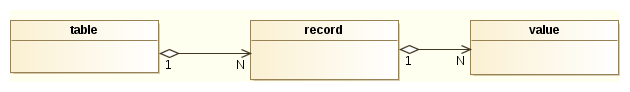
\includegraphics{pics/record_reader_model.png}}
\end{figure}

In this final section a typical use-case for a type erasure will be discussed. 
One problem that regularly pops up is the reading of tabular ASCII data. 
The file {\tt record.dat} in the examples directory shows such data
\inputminted[fontsize=\small,
             frame=lines,
             label=examples/record.dat]
{text}{../examples/record.dat}
While the elements of the first two columns are integer and float respectively,
the third column holds complex numbers. There are several ways how to approach
this problem. The first would be to use a C-style {\tt struct} or a class to
keep the values of each column together. However, this is a quite static
approach and would not help if the data type of each column has to be determined
at runtime. 

In this example a different approach with a type erasure is used. 
The complete code of the example can be found in {\tt type\_erasure\_record.cpp}
in the example directory of the source distribution.
\inputminted[linenos,
             fontsize=\small,
             firstnumber=26,
             firstline=26,
             lastline=36,
             frame=lines,
             label=examples/type\_erasure\_record.cpp
             ]
{cpp}{../examples/type_erasure_record.cpp}
The data we would like to read is a table which can be considered as a container
of record. The two types are defined in lines $35$ and $36$. Before we have a
look at the implementation of the individual functions lets have a look at the
main program
\inputminted[linenos,
             fontsize=\small,
             firstnumber=93,
             firstline=93,
             lastline=106,
             frame=lines,
             label=examples/type\_erasure\_record.cpp
             ]
{cpp}{../examples/type_erasure_record.cpp}
which produces the following output
\begin{minted}[fontsize=\small,frame=lines]{bash}
INT32
FLOAT64
COMPLEX32
11      -123.23 (-1,0.23)
13      -12.343 (12.23,-0.2)
16      134.12  (1.23,-12.23)
\end{minted}
The main program has the following sections: in lines $95$ and $97$ the file
is opened and the data read. Lines $100$ to $101$ print the data types of the
elements in the first row and line $100$ prints the content of the file to
standard output.
Lets first have a look on the {\tt read\_table} implementation.
\inputminted[linenos,
             fontsize=\small,
             firstnumber=56,
             firstline=56,
             lastline=72,
             frame=lines,
             label=examples/type\_erasure\_record.cpp
             ]
{cpp}{../examples/type_erasure_record.cpp}
The main loop starts at line $64$ and is rather straight forward. With every
iteration a single line is read from the file and basically passed to the {\tt
read\_record} function (if it is not empty). 
The really interesting part comes in the {\tt read\_record} function:
\inputminted[linenos,
             fontsize=\small,
             firstnumber=38,
             firstline=38,
             lastline=54,
             frame=lines,
             label=examples/type\_erasure\_record.cpp
             ]
{cpp}{../examples/type_erasure_record.cpp}
In line $48$ the individual data entries are read and pushed into the record
vector in lines $49$ to $51$ by passing the typed variables to a type erasure. 
This is virtually the only way to store elements of different type in a {\tt
std::vector}.
\inputminted[linenos,
             fontsize=\small,
             firstnumber=74,
             firstline=74,
             lastline=81,
             frame=lines,
             label=examples/type\_erasure\_record.cpp
             ]
{cpp}{../examples/type_erasure_record.cpp}

\inputminted[linenos,
             fontsize=\small,
             firstnumber=83,
             firstline=83,
             lastline=89,
             frame=lines,
             label=examples/type\_erasure\_record.cpp
             ]
{cpp}{../examples/type_erasure_record.cpp}

